\chapter{Introduction}
\label{introduction}

%intro to the intro here


\section{Motivation}

%expanded version of the above? need stats on depression and schizophrenia
It is estimated that disorders of the brain cost Europe €798 billion Euros in 2010\autocite{olesen_economic_2012}.
Specifically, depression is estimated to cost Europe €91.9 billion in 2004 and schizophrenia along with associated psychotic disorders is estimated at €93.9 billion.
There are many diseases with currently limited treatment options in the brain, and a deeper understanding of the brain is required to treat them. 

%FIN: even in motivation say why proteins matter to understanding brain - key components, molecular machines etc

These diseases are very likely to act at the synaptic level\autocites{chua_architecture_2010,synsys}.
However, the exact proteins or genes involved in these diseases are unknown.
If it is possible to even gain slightly more information about associated proteins at the synapse it may be possible to develop new treatments\autocite{li_interaction_2010}.

In addition, as a project this includes work from various areas, such as Bioinformatics, Machine Learning and Software Development that made it a good learning exercise. %FIN: thus made it a good 
It is a worthwhile investment in the fundamentals of constructing PPI networks. %FIN: first usage of acronym should be in full, Protein-Protein Interaction 

%overview of the project or the report? pretty sure it's the report
\section{Outline}
%sections to cover:
% background
% methods
% results
% conclusion

This project involved combining both direct and indirect data sources to create weighted edges in a PPI graph to affect the communities detected by a Community Detection algorithm.
A flow chart describing this process and the elements involved is shown in figure \ref{fig:expflow}.
There are three main input sources shown, the pull-down experiments, direct data and indirect data.
%FIN: worth briefly explaining what pull-down experiments are or their importance i.e. that they are potentially empirical molecular validation of protein-protein interaction predictions
Pull-down experiments were used to identify the proteins of interest, which were used to build an interaction network using direct data sources, such as interaction databases.
The indirect data sources, such as functional annotations of proteins, were used along with direct data sources in the process to generate weighted graphs.

%flow charts from the proposal could go here
\begin{figure}
    \centering
    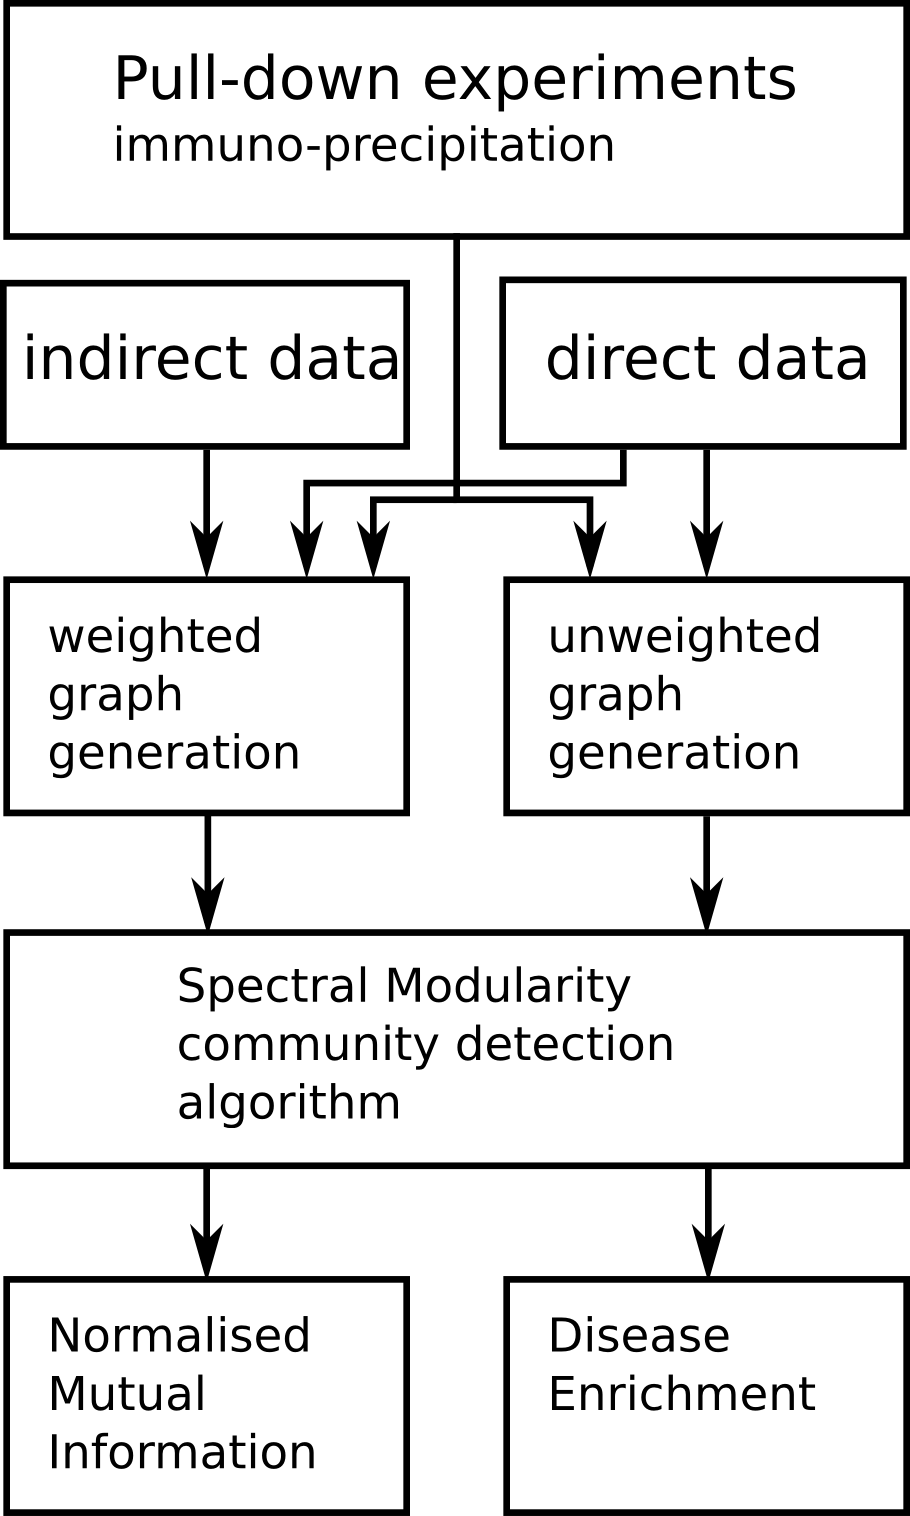
\includegraphics[width=0.6\textwidth]{expflow.png}
    \caption{A flow chart describing how the elements of the project as a whole, as shown in the project proposal.}
    \label{fig:expflow}
\end{figure}

The resulting weighted and unweighted PPI graphs were then separated into communities using a Community Detection algorithm.
These communities could then be compared using the two methods named in figure \ref{fig:expflow}: Disease Enrichment and NMI.
The results of these tested the hypothesis of the project. %FIN: "results of these were used to test" is clearer

%hypothesis required %FIN: hypothesis needs stated earlier - this is a bit confusing
The hypothesis of this project was that the communities detected in each case would differ and that these differences would be relevant to the conclusions each network could illustrate about a particular disease.
NMI was able to show simply that the two sets of communities detected was different. %FIN: were different
Disease enrichment refers to testing the likelihood that a given community is involved in a particular disease. %FIN: for example? You would expect a community to represent a certain cluster of interacting proteins right? 
%FIN: they identify a high confidence interaction network/cluster around known Alzheimer's related proteins and identify putative additional factors  Genome Res. 2011 Mar;21(3):364-76. doi: 10.1101/gr.114280.110. Epub 2010 Dec 16.
%FIN: Interactome mapping suggests new mechanistic details underlying Alzheimer's disease.
%FIN: Soler-López M1, Zanzoni A, Lluís R, Stelzl U, Aloy P.
This allowed us to show the differences in the predictions for disease involvement given by each network due to the weighting of the networks.
%FIN:this sentence is horrific - split it or rephrase

%structure of the report and other resources
The report first describes the background knowledge driving the hypothesis of the project in chapter \ref{background}.
In chapter \ref{methods} the methods involved in executing the project are described.
Finally, the results obtained are described in chapter \ref{results}.
In addition, the execution of all commands required to reproduce the project were recorded in notebooks described in section \ref{app:notebooks}.
This project was stored in a git repository and is publicly available in a repository described in Appendix \ref{app:repository}.

%progress flow charts from the proposal could go here, or above

%could also include one updated to reflect the real project

%should also mention the prototype run through and which week it occurred in 

\section*{Conclusion}

The following report covers the background information necessary to understand the methods of the project and the results which were obtained.
It was approached as an opportunity to use a variety of new tools, and each will be described as the report continues. %FIN: "an opportunity to investigate the effectiveness of new tools in resolving known issues in predicting PPI" or something like that
